\chapter{آزمایش‌ها و نتایج}
\label{ch:results}

برای هر نتیجه، مقدار، مخرج و مرز ادعای مجاز مشخص شده است. همه اعداد از
مصنوعات ثبت‌شده خوانده شده‌اند.

\section{پوشش شروط پذیرش و وضعیت شواهد}
\label{sec:res-gates}

جدول~\ref{tab:gates} وضعیت شواهد شروط پذیرش را نشان می‌دهد. پنج شرط از نه
شرط شواهد کافی دارند و برای چهار شرط شواهد تکمیلی لازم است. این وضعیت
به کفایت شواهد هر شرط مربوط است و نباید با آمادگی خود گزارش برای ارائه و
داوری یکسان دانسته شود.

\begin{table}[ht]
\centering
\caption{پوشش شروط پذیرش پروژه}
\label{tab:gates}
\small
\begin{tabular}{L{8.4cm}c}
\toprule
\textbf{شرط پذیرش} & \textbf{وضعیت شواهد} \\
\midrule
نمونه اولیه کارکردی گفتار‌به‌گفتار فارسی & کافی \\
عبور از آزمون نهایی معنایی خودکار & کافی \\
خروجی ممیزی‌شده در بازه \N{100} تا \N{200} ساعت & کافی \\
حل‌شدن سیاست داده تحت انصراف مستند بازبینی & کافی \\
انتخاب مجوز کد منبع & کافی \\
\midrule
مدل مستقیم فارسی واجد شرایط استقرار & نتیجه مثبت تازه لازم است \\
آشکارساز با دقت بیش از \N{80} درصد روی برچسب مستقل & شواهد تکمیلی لازم است \\
تناسب و تأخیر زنده روی سخت‌افزار \N{12} تا \N{24} گیگابایتی & شواهد تکمیلی لازم است \\
تکمیل مطالعه انسانی & شواهد تکمیلی لازم است \\
\bottomrule
\end{tabular}
\end{table}

\مرزادعا{پنج شرط مهندسی شواهد کافی دارند. چهار ردیف پایانی هنوز به نتیجه
مثبت یا شواهد رسمی تکمیلی نیاز دارند؛ برای نتایج اثبات‌نشده ادعای قطعی
مطرح نمی‌شود.}

\section{مجموعه داده}
\label{sec:res-data}

جدول~\ref{tab:corpus} مشخصات نهایی را نشان می‌دهد. مقدار \N{108.584} ساعت
درون بازه ن۴ است و ممیزی خودکار یکپارچگی، شامل ترتیب کانال‌ها، درهم‌سازی و
تفکیک گروهی، بدون شکست گذشته است.

\begin{table}[ht]
\centering
\caption{مشخصات مجموعه داده مکالمه فارسی مشتق‌شده}
\label{tab:corpus}
\small
\begin{tabular}{L{7.6cm}R{3.2cm}}
\toprule
\textbf{شاخص} & \textbf{مقدار} \\
\midrule
موجودی زیرنویس کانال‌ها & \N{775.887} ساعت \\
جفت‌های پاسخ بدون بازاستفاده & \N{6,754} \\
ساعت صوت منبع جفت‌ها & \N{123.796} ساعت \\
گویندگان / نشست‌ها & \N{407/162} \\
ساعت استریوی خروجی & \N{108.584} ساعت \\
تفکیک آموزش / اعتبارسنجی / آزمون & \N{6,419/131/204} \\
نشت گروهی / شکست ممیزی خودکار & \N{0/0} \\
نامزدهای خودکار رخداد تعاملی & \N{770} \\
ردیف‌های تأییدشده توسط انسان & \N{0} \\
\bottomrule
\end{tabular}
\end{table}

\مرزادعا{برچسب‌های تعاملی نامزد خودکارند. این مجموعه را نمی‌توان
برچسب‌گذاری‌شده توسط انسان نامید و داده منبع قابل بازنشر نیست.}

\section{سامانه آبشاری: پنل مکانیکی و فهم‌پذیری}
\label{sec:res-cascade}

پنل اعتبارسنجی، ۹ ردیف با فاصله ثابت از فهرست‌نامه \N{131} ردیفی است. شاخص
ردیف‌ها پیش از اجرا قفل بود. زنجیره، سرویس واقعی بازشناسی، پاسخ‌گوی
\en{Qwen2.5-0.5B-Instruct} و موتور گفتاری واقعی است و ورودی کانال یک
ممیزی‌شده کاربر است. این پنل مکانیک زنجیره را می‌سنجد، نه کیفیت معنایی
\en{Qwen3-4B}. نتیجه در جدول~\ref{tab:cascade-panel} آمده است.

\begin{table}[ht]
\centering
\caption{نتیجه پنل ثابت اعتبارسنجی سامانه آبشاری}
\label{tab:cascade-panel}
\small
\begin{tabular}{L{7.8cm}R{3.0cm}}
\toprule
\textbf{شاخص} & \textbf{مقدار} \\
\midrule
پاسخ‌گوی متنی پنل & \en{Qwen2.5-0.5B} \\
ردیف‌های عبور‌کرده از همه شروط & \N{9/9} \\
ردیف‌های با پاسخ جایگزین قاعده‌محور & \N{0/9} \\
کمینه سهم نویسه فارسی در رونویسی و پاسخ & \N{1.000} \\
پاسخ‌های صوتی غیرساکت & \N{9/9} \\
کمینه ریشه میانگین مربعات صوت پاسخ & \N{0.133529} \\
میانه / بیشینه زمان تولید کامل (ms) & \N{5584.7/13270.2} \\
ردیف‌های آزمون نهایی استفاده‌شده & \N{0} \\
\bottomrule
\end{tabular}
\end{table}

میانه، صدک نود‌و‌پنجم و بیشینه طول رونویسی \N{445}، \N{3977.8} و
\N{5031} نویسه بود. همبستگی پیرسون توصیفی میان طول رونویسی و زمان تولید
کامل \N{0.885} است؛ بلندترین رونویسی و کندترین نوبت هر دو ردیف \N{32}
بودند. ستون زمان، مدت تولید کامل پاسخ است نه تأخیر نخستین صوت.

بازبازشناسی همان ۹ خروجی، با متن پاسخ به‌عنوان مرجع، نرخ خطای نویسه تجمیع
خرد \N{7.14} درصد (\N{47/658}) و نرخ خطای واژه \N{30.41} درصد
(\N{52/171}) را نشان داد. هیچ ردیفی تطابق کامل واژه‌ای یا نویسه‌ای نداشت.
شکل~\ref{fig:cascade} هر دو محور را نشان می‌دهد.

\begin{figure}[ht]
\centering
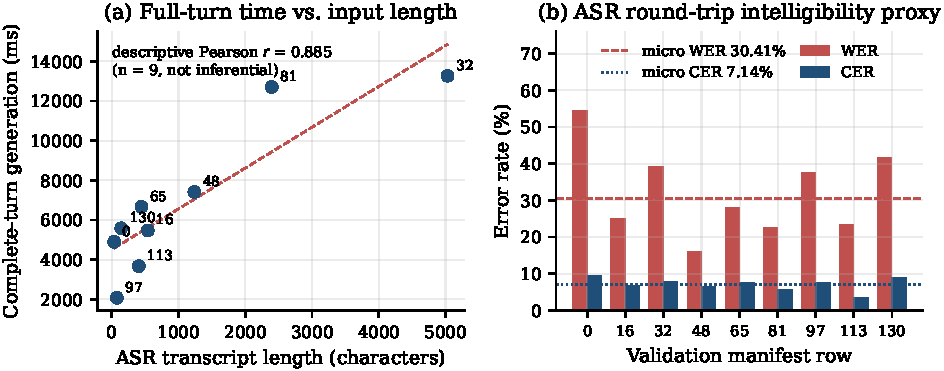
\includegraphics[width=0.96\textwidth]{figs/cascade_panel.pdf}
\caption{(الف) زمان تولید کامل در برابر طول رونویسی برای ۹ ردیف پنل.
         (ب) نرخ خطای واژه و نویسه بازبازشناسی همان ۹ خروجی.}
\label{fig:cascade}
\end{figure}

\مرزادعا{نتیجه مکانیکی برون‌نمونه با پاسخ‌گوی \en{Qwen2.5-0.5B} است و به
\en{Qwen3-4B} تعمیم داده نمی‌شود. نُه ردیف برای تعمیم جمعیتی کافی نیست.
زمان تولید کامل سنجه $T_{\text{first\_audio}}$ نیست و شرط \N{500} میلی‌ثانیه
را برآورده نمی‌کند. بازبازشناسی فهم‌پذیری انسانی یا طبیعی‌بودن را اثبات
نمی‌کند.}

\section{آزمون معنایی خودکار}
\label{sec:res-semantic}

مرحله صلاحیت روی هفت ردیف اعتبارسنجی استفاده‌نشده همه شروط را گذراند:
\N{42/42} فراخوانی معتبر، ارتباط \N{3.857} در برابر \N{1.000}، انسجام
\N{3.571}، برد زوجی \N{6/7} و ارتباط حداقل دو \N{100} درصد. تنها پس از این
عبور، آزمون نهایی یک‌بار باز شد.

آزمون نهایی روی \N{40} ردیف از فهرست‌نامه \N{204} ردیفی و در پنج نشست کنارگذاشته
اجرا شد. سه بازوی دوسوکور: خط پایه قفل‌شده \en{Qwen2.5-0.5B}، نامزد
\en{Qwen3-4B} با پرامپت \en{v2}، و مرجع هم‌ترازشده خودکار نوبت بعدی. داور
\en{Qwen3.8-27B-FP8} با دمای صفر و دو تکرار در هر ردیف بود.
جدول~\ref{tab:semantic} نتیجه را نشان می‌دهد و
جدول~\ref{tab:semantic-gates} عبور هر هفت شرط ازپیش‌تعریف‌شده را.

\begin{table}[ht]
\centering
\caption{نتیجه آزمون نهایی معنایی خودکار روی \N{40} ردیف گروه‌ناهمپوشان}
\label{tab:semantic}
\small
\begin{tabular}{L{6.6cm}R{4.2cm}}
\toprule
\textbf{شاخص} & \textbf{مقدار} \\
\midrule
فراخوانی معتبر داور / مورد انتظار & \N{240/240} \\
نرخ توافق تکرار داور & \N{1.00} \\
میانگین ارتباط نامزد / خط پایه / مرجع & \N{3.150/1.425/0.950} \\
میانگین انسجام نامزد / خط پایه & \N{3.325/1.525} \\
بهبود ارتباط / انسجام نسبت به خط پایه & \N{+1.725/+1.800} \\
برد زوجی ارتباط & \N{27/40} (\N{67.5\%}) \\
ارتباط حداقل دو & \N{35/40} (\N{87.5\%}) \\
تلاش دوباره تولید / صوت نامعتبر نامزد & \N{0/0} \\
\bottomrule
\end{tabular}
\end{table}

\begin{table}[ht]
\centering
\caption{شروط خودکار ازپیش‌تعریف‌شده آزمون نهایی}
\label{tab:semantic-gates}
\small
\begin{tabular}{L{5.8cm}rrc}
\toprule
\textbf{شرط} & \textbf{آستانه} & \textbf{مشاهده} & \textbf{وضعیت} \\
\midrule
میانگین ارتباط نامزد & $\ge$ \N{2.00} & \N{3.150} & برآورده \\
میانگین انسجام نامزد & $\ge$ \N{2.50} & \N{3.325} & برآورده \\
بهبود ارتباط & $\ge$ \N{0.50} & \N{1.725} & برآورده \\
بهبود انسجام & $\ge$ \N{0} & \N{1.800} & برآورده \\
نرخ برد زوجی ارتباط & $\ge$ \N{0.60} & \N{0.675} & برآورده \\
نرخ ارتباط حداقل دو & $\ge$ \N{0.70} & \N{0.875} & برآورده \\
اعتبار کامل مکانیکی & \N{240/240} & \N{240/240} & برآورده \\
\bottomrule
\end{tabular}
\end{table}

شکل~\ref{fig:semantic} میانگین و توزیع امتیازها را نشان می‌دهد. امتیاز پایین
مرجع هم‌ترازشده نشان می‌دهد که «گفتن نوبت بعدی پیکره» لزوماً پاسخ مناسب به
اظهار کاربر نیست.

\begin{figure}[ht]
\centering
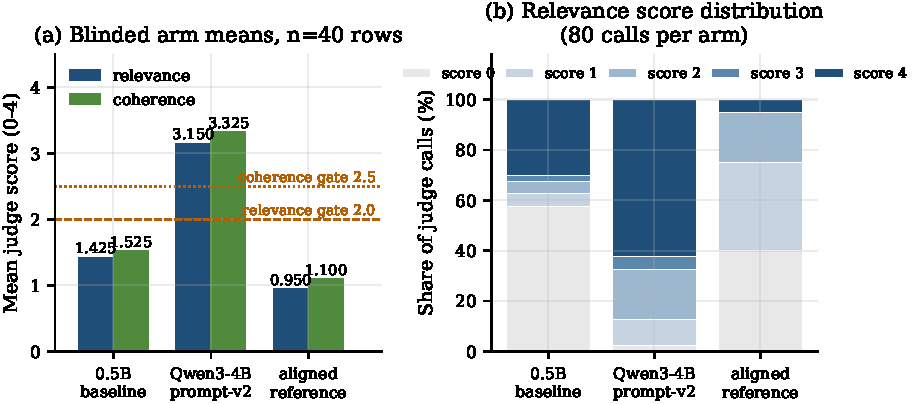
\includegraphics[width=0.96\textwidth]{figs/semantic_final_test.pdf}
\caption{(الف) میانگین ارتباط و انسجام سه بازوی دوسوکور.
         (ب) توزیع امتیاز ارتباط در \N{80} فراخوانی داور برای هر بازو.}
\label{fig:semantic}
\end{figure}

یک آزمایش جانبی \en{LoRA} روی پاسخ‌گو زیان توسعه را \N{31.18} درصد کاهش داد
اما در ارزیابی معنایی از خط پایه پیشی نگرفت و در سامانه نهایی به کار نرفت.

\مرزادعا{عبور از هفت شرط خودکار به معنای کیفیت ادراکی یا معیار مستقل نیست.
داور و نامزد هم‌خانواده‌اند.}

\section{تشخیص وقفه و پیوستگی انتقال}
\label{sec:res-bargein}

روی داده مصنوعی، طبقه‌بند روی \N{32} نمونه کنارگذاشته به دقت \N{1.000}
رسید؛ این عدد تنها آزمون بازگشتی است، چون داده مصنوعی از همان مدل تولیدی
ساخته شده که ویژگی‌ها را جداپذیر می‌کند.

ارزیابی معنادار روی رخدادهای صوت واقعی بود. آستانه \N{0.70} تنها روی
\N{24} نشست اعتبارسنجی انتخاب و یک‌بار روی \N{22} نشست آزمون با
\N{132} رخداد اعمال شد (جدول~\ref{tab:bargein}). ماتریس درهم‌ریختگی:
\N{60} منفی درست، \N{6} مثبت نادرست، \N{19} منفی نادرست و \N{47} مثبت درست.

\begin{table}[ht]
\centering
\caption{تقریب آشکارساز وقفه روی رخدادهای صوت ضبط‌شده با نشست کنارگذاشته}
\label{tab:bargein}
\small
\begin{tabular}{L{3.2cm}rrl}
\toprule
\textbf{سنجه} & \textbf{آشکارساز} & \textbf{خط پایه} &
\textbf{فاصله اطمینان \N{95\%}} \\
 & \textbf{پیشنهادی} & \textbf{انرژی} & \textbf{(بلوکی، نشست)} \\
\midrule
دقت & \N{81.06\%} & \N{78.03\%} & \N{74.44\% -- 87.18\%} \\
امتیاز \en{F1} وقفه & \N{78.99\%} & \N{71.84\%} & \N{72.34\% -- 85.71\%} \\
نرخ پذیرش نادرست & \N{9.09\%} & \N{0.00\%} & \N{2.63\% -- 16.92\%} \\
نرخ رد نادرست & \N{28.79\%} & \N{43.94\%} & \N{19.30\% -- 37.23\%} \\
\bottomrule
\end{tabular}
\end{table}

آزمون بازگشتی بستر \en{WebSocket} با چهار آزمون گذشت. ممیزی مخزن
\N{206} آزمون موفق، پوشش شاخه‌ای \N{65} درصد و بررسی نوع بدون خطا روی
\N{49} پرونده را ثبت کرد.

\مرزادعا{دقت نقطه‌ای \N{81.06} درصد از \N{80} درصد بالاتر است، اما کران
پایین فاصله اطمینان بلوکی نشست \N{74.44} درصد است. برچسب‌ها از تفکیک
گوینده خودکارند. بنابراین ن۵ اثبات نشده است. ن۲ به‌صورت نرم‌افزاری برآورده
و به‌صورت رسمی اثبات‌نشده است.}

\section{مسیر مستقیم}
\label{sec:res-moshi}

جدول~\ref{tab:moshi-summary} شش نسل را خلاصه می‌کند. الگوی مشترک: زیان کاهش
می‌یابد و شرط اجرا برآورده نمی‌شود. مقادیر کمینه زیان میان نسل‌ها مستقیماً
قابل مقایسه نیستند، چون پنجره و مجموعه ارزیابی فرق دارد. برای \en{v6.2}
زیان درون‌نمونه است.

\begin{table}[ht]
\centering
\caption{خلاصه شش نسل مسیر مستقیم. «بهترین اجرا» بیشترین شمار ردیف عبور‌کرده
         از ۹ ردیف در میان چک‌پوینت‌های آن نسل است.}
\label{tab:moshi-summary}
\small
\begin{tabular}{lrrrrc}
\toprule
\textbf{نسخه} & \textbf{پنجره} & \textbf{نامزد} & \textbf{کمینه} &
\textbf{بهترین} & \textbf{واجد} \\
 & \textbf{(ثانیه)} & & \textbf{زیان} & \textbf{اجرا} & \textbf{شرایط} \\
\midrule
\en{v1}   & \N{20}  & \N{16} & \N{1.402} & \N{0/9} & نه \\
\en{v2}   & \N{100} & \N{20} & \N{1.735} & \N{2/9} & نه \\
\en{v3}   & \N{100} & \N{5}  & \N{1.879} & \N{1/9} & نه \\
\en{v4}   & \N{100} & \N{5}  & \N{1.879} & \N{1/9} & نه \\
\en{v5}   & \N{100} & \N{5}  & \N{1.868} & \N{1/9} & نه \\
\en{v6.2} & \N{12}  & \N{4}  & \N{2.060} & \N{0/9} & نه \\
\bottomrule
\end{tabular}
\end{table}

در \en{v6.2} بهترین زیان متنی پس از گام \N{50} برابر \N{0.550852} است که
\N{32.20} درصد کمتر از \N{0.812474} در گام \N{50} است و از معیار
\N{30} درصد بالاتر می‌رود؛ یعنی آداپتر ظرفیت برازش هدف را دارد. با این حال
هر چهار چک‌پوینت \N{0} از \N{9} گرفتند و در هر چک‌پوینت تنها یک ردیف از نه
ردیف هم‌زمان متن و گفتار تولید کرد. شکل~\ref{fig:trials} این دو محور را در
برابر هم می‌گذارد.

\begin{figure}[ht]
\centering
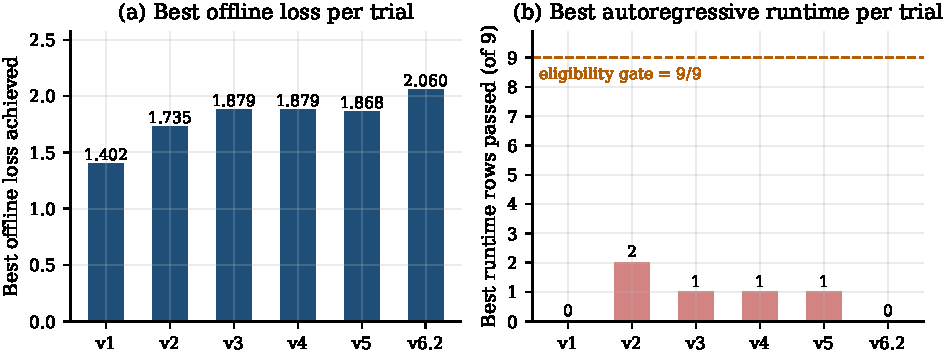
\includegraphics[width=0.96\textwidth]{figs/moshi_trials_summary.pdf}
\caption{(الف) بهترین زیان آفلاین هر نسل. (ب) بیشترین شمار ردیف عبور‌کرده از
         پنل اجرا، در برابر شرط \N{9/9}.}
\label{fig:trials}
\end{figure}

\مرزادعا{هیچ چک‌پوینتی واجد شرایط استقرار نیست. عبارت «مدل \en{Moshika} با
موفقیت برای فارسی تنظیم شد» با این شواهد نادرست است.}

\section{تأخیر، سخت‌افزار و مطالعه انسانی}
\label{sec:res-unmet}

سخت‌افزار موجود \en{NVIDIA H100 NVL} با \N{93.09} گیگابایت حافظه بود که از
بازه ن۶ خارج است. سقف نرم‌افزاری حافظه، کارت \N{93} گیگابایتی را به کارت
\N{24} گیگابایتی تبدیل نمی‌کند. شمار ردیف‌های واجد شرایط رسمی سرتاسری صفر
است. میانه زمان تولید کامل در پنل مکانیکی \N{5584.7} میلی‌ثانیه است. میانه
زمان‌سنجی سمت سرور برای توقف پخش بدون سقف حافظه \N{11.71} میلی‌ثانیه بود؛
این مقدار تأیید پخش مرورگر ندارد و سنجه سرتاسری نیست.

پروتکل مطالعه انسانی، رضایت‌نامه و برگه امتیازدهی در مخزن ثبت شد. اجرا تکمیل
نشد: یک شرکت‌کننده، یک نفر بالای \N{60} سال، و \N{0} مجموعه امتیاز کامل.
مخرج امتیازدهی صفر است.

\مرزادعا{ادعای «تأخیر سامانه کمتر از \N{500} میلی‌ثانیه است» مجاز نیست.
هیچ ادعایی درباره طبیعی‌بودن، رضایت کاربری یا تجربه سالمندان مطرح نمی‌شود.}

\section{وضعیت نهایی نیازمندی‌ها}
\label{sec:res-requirements}

\begin{table}[ht]
\centering
\caption{وضعیت نهایی هفت نیازمندی تعریف پروژه}
\label{tab:req-status}
\small
\begin{tabular}{cL{4.2cm}L{5.4cm}}
\toprule
\textbf{شماره} & \textbf{وضعیت} & \textbf{شواهد پشتیبان} \\
\midrule
ن۱ & برآورده برای مسیر آبشاری &
     پنل ثابت \N{9/9} با صفر پاسخ جایگزین \\
ن۲ & نرم‌افزاری برآورده، رسمی اثبات‌نشده &
     چهار آزمون بازگشتی بستر؛ بدون مرورگر فیزیکی \\
ن۳ & اندازه‌گیری رسمی انجام نشده &
     صفر ردیف واجد شرایط سرتاسری \\
ن۴ & برآورده &
     \N{108.584} ساعت خروجی ممیزی‌شده \\
ن۵ & پیاده‌سازی‌شده، عبور رسمی اثبات‌نشده &
     دقت \N{81.06\%} با برچسب خودکار؛ کران پایین \N{74.44\%} \\
ن۶ & شواهد رسمی موجود نیست &
     سخت‌افزار موجود \N{93.09} گیگابایتی \\
ن۷ & شواهد رسمی موجود نیست &
     یک شرکت‌کننده، صفر مجموعه امتیاز کامل \\
\bottomrule
\end{tabular}
\end{table}

\مرزادعا{ن۱ در این جدول تنها عبور مکانیکی \N{9/9} با پاسخ‌گوی
\en{Qwen2.5-0.5B} را پوشش می‌دهد. ن۳، ن۵، ن۶ و ن۷ اثبات نشده‌اند.}

از چهار قلم خروجی مورد انتظار، سه قلم تولید و مستند شده‌اند: نمونه اولیه
آبشاری، کد منبع مستند، و مجموعه داده مکالمه فارسی. برای قلم چهارم،
پروتکل و زیرساخت سنجش آماده است؛ یافته‌های تجربی تعامل سالمندان تنها پس
از تکمیل مطالعه انسانی قابل گزارش خواهد بود.
